\documentclass{homework}

\input{particulars}

\sisetup{round-precision=3}

\renewcommand\thesection{\arabic{section}}
\renewcommand\thesubsection{\thesection.\arabic{subsection}}
\renewcommand\thesubsubsection{\thesubsection.\arabic{subsubsection}}

\begin{document}

\title{Machine Learning Homework \#7}
\author{\chineseName \masterStudentID}
\date{}
\maketitle

\section{Code with detailed explanations}

\subsection{Kernel Eigenfaces}

\subsubsection{Part 1}

All the code below is written in p1.ipynb.

The imported modules are:

\begin{lstlisting}[language=Python]
import cv2
import os
import matplotlib.pyplot as plt
import numpy as np
\end{lstlisting}

Here is the code for loading the images:

\begin{lstlisting}[language=Python]
def load_images(folder_path, size_factor=1):
    """
    Read .pgm images from a folder and return images, labels(extracted from file names), facial expressions and image shape.
    The image will be resized by size_factor.
    """
    images = []
    labels = []
    facial_expressions = []
    for file in os.listdir(folder_path):
        if file.endswith(".pgm"):
            img_path = os.path.join(folder_path, file)
            img = cv2.imread(img_path, cv2.IMREAD_GRAYSCALE)
            img = cv2.resize(img, (0, 0), fx=size_factor, fy=size_factor)
            images.append(img)
            labels.append(int(file.split(".")[0][7:]) - 1)
            facial_expressions.append(file.split(".")[1])
    images = np.array(images)
    image_shape = images[0].shape
    images = images.reshape(images.shape[0], images.shape[1] * images.shape[2])
    labels = np.array(labels)
    facial_expressions = np.array(facial_expressions)
    return images, labels, facial_expressions, image_shape

size_factor = 0.5
train_images, train_labels, _, image_shape = load_images("Yale_Face_Database/Training", size_factor=size_factor)
test_images, test_labels, _, _ = load_images("Yale_Face_Database/Testing", size_factor=size_factor)
\end{lstlisting}

The code for PCA is shown below. The calculation steps is written in the code comments.

\begin{lstlisting}[language=Python]
def PCA(images, n_components=50):
    # Calculate the mean face by averaging the images
    mean_face = np.mean(images, axis=0)
    # Center the data
    centered_data = images - mean_face

    # Compute the reduced covariance matrix
    # Because the number of samples is smaller than the number of features, we can use the reduced formula
    cov_reduced = np.dot(centered_data, centered_data.T) / images.shape[0]

    # Eigen decomposition of the reduced covariance matrix
    eigvals, eigvecs = np.linalg.eigh(cov_reduced)

    # Sort eigenvectors by eigenvalues in descending order
    sorted_indices = np.argsort(eigvals)[::-1]
    eigvals = eigvals[sorted_indices]
    eigvecs = eigvecs[:, sorted_indices]

    # Compute the original eigenvectors
    eigvecs_full = np.dot(centered_data.T, eigvecs)
    eigvecs_full = eigvecs_full / np.linalg.norm(eigvecs_full, axis=0)  # Normalize

    # Select the top n_components, it also return the eigenvalues and the mean face
    return eigvecs_full[:, :n_components], eigvals[:n_components], mean_face


# Compute Eigenfaces
eigenfaces, eigenvalues, mean_face = PCA(train_images, n_components=200)
\end{lstlisting}

The code for LDA is shown below. The calculation steps is written in the code comments.

\begin{lstlisting}[language=Python]
def LDA(images, labels, n_components=None):
    N = images.shape[1]
    # Calculate the mean face by averaging the images
    mean_face = np.mean(images, axis=0)
    Sw = np.zeros((N, N))
    Sb = np.zeros((N, N))
    # Get unique labels
    unique_labels = np.unique(labels)
    mean_classes = np.zeros((len(unique_labels), N))
    class_count = np.zeros(len(unique_labels))

    # Calculate the mean of each classes
    for i in unique_labels:
        class_images = images[labels == i]
        class_count[i] = class_images.shape[0]
        mean_classes[i] = np.mean(class_images, axis=0)
    print(f"mean_classes: {mean_classes[0].max(), mean_classes[0].min()}")

    # Calculate the distance within-class scatter
    print("Computing Sw")
    for i in unique_labels:
        d = images[labels == i] - mean_classes[i]
        Sw += d.T @ d

    # Calculate the distance between-class scatter
    print("Computing Sb")
    for i in unique_labels:
        d = (mean_classes[i] - mean_face).reshape(-1, 1)
        Sb += class_count[i] * (d @ d.T)

    print(f"Sw shape: {Sw.shape}")
    print(f"Sb shape: {Sb.shape}")
    # Solve the generalized eigenvalue problem for LDA
    eigenvalues, eigenvectors = np.linalg.eig(np.linalg.inv(Sw) @ Sb)

    # Sort eigenvalues and eigenvectors in descending order
    sort_index = np.argsort(-eigenvalues)

    # Select the top k eigenvectors and eigenvalues
    # If n_components is not set, n_components = len(sort_index) - 1 because the last eigenvector is 0
    if n_components is None:
        n_components = len(sort_index) - 1
    sort_index = sort_index[:n_components]

    eigenvalues = np.asarray(eigenvalues[sort_index].real, dtype="float")
    eigenvectors = np.asarray(eigenvectors[:, sort_index].real, dtype="float")

    # Return the eigenvalues and eigenvectors
    return eigenvalues, eigenvectors


# project the images to the PCA subspace to reduce the dimensionality
train_images_pca = np.dot(train_images - mean_face, eigenfaces)
# Compute Fisherfaces in the PCA subspace
fishervalues, fisherfaces, = LDA(train_images_pca, train_labels)
# Compute Fisherfaces in the original space
fisherfaces = np.dot(eigenfaces, fisherfaces)
\end{lstlisting}

Here is the code for visualize the eigenfaces and fisherfaces:

\begin{lstlisting}[language=Python]
# Visualize Eigenfaces
height = 1
width = image_shape[1] / image_shape[0]
fig, axes = plt.subplots(5, 5, figsize=(width * 5, height * 5))
axes = axes.flatten()
for i in range(25):
    axes[i].imshow(eigenfaces[:, i].reshape(image_shape), cmap="gray")
    axes[i].axis("off")
plt.subplots_adjust(wspace=0, hspace=0)
plt.show()

# Visualize Fisherfaces
multiple = 1
figheight = 1 * 5
figwidth = image_shape[1] / image_shape[0] * 5
figsize = (figwidth * multiple, figheight * multiple)
fig, axes = plt.subplots(5, 5, figsize=figsize)
axes = axes.flatten()

for i in range(25):  # Visualize first 5 fisherfaces
    axes[i].imshow(fisherfaces[:, i].reshape(image_shape), cmap="gray")
    axes[i].axis("off")
plt.subplots_adjust(wspace=0, hspace=0)
plt.show()
\end{lstlisting}

The code for reconstructing and visualizing the images is shown below. For test images and LDA method, the code is similar.

\begin{lstlisting}[language=Python]
def reconstruct_images(images, eigenfaces, mean_face):
    # Center the data
    centered_data = images - mean_face
    # Compute the projected data
    weights = np.dot(centered_data, eigenfaces)
    # Reconstruct the data and add the mean face
    reconstructed_data = mean_face + np.dot(weights, eigenfaces.T)
    return reconstructed_data

# Randomly select 10 images from the training set
np.random.seed(42)
n_images = 10
train_images_sample = train_images[np.random.choice(train_images.shape[0], n_images, replace=False)]
train_reconstructed_images = reconstruct_images(train_images_sample, eigenfaces, mean_face)

# Visualize original and reconstructed images
multiple = 3
figheight = 1 * 2
figwidth = image_shape[1] / image_shape[0] * n_images
figsize=(figwidth * multiple, figheight * multiple)
fig, axes = plt.subplots(2, n_images, figsize=figsize)
axes = axes.flatten()

for i in range(n_images):
    # Original image
    axes[i].imshow(train_images_sample[i].reshape(image_shape), cmap='gray')
    axes[i].set_title("Original")
    axes[i].axis('off')
    
    # Reconstructed image
    axes[i + n_images].imshow(train_reconstructed_images[i].reshape(image_shape), cmap='gray')
    axes[i + n_images].set_title("Reconstructed")
    axes[i + n_images].axis('off')

plt.subplots_adjust(wspace=0, hspace=0.2)
plt.show() 
\end{lstlisting}

\subsubsection{Part 2}

The code for KNN algorithm is shown below:

\begin{lstlisting}[language=Python]
def k_nearest_neighbors(X_train, y_train, X_test, k=3):
    y_pred = []
    for test_point in X_test:
        # Compute Euclidean distances to all training points
        distances = np.sqrt(np.sum((X_train - test_point) ** 2, axis=1))
        # Get the indices of the k nearest neighbors
        neighbors_idx = np.argsort(distances)[:k]
        # Get the labels of the k nearest neighbors
        neighbors_labels = y_train[neighbors_idx]
        # predict the most frequent label
        unique, counts = np.unique(neighbors_labels, return_counts=True)
        y_pred.append(unique[np.argmax(counts)])
    return np.array(y_pred)
\end{lstlisting}

The code for calculating the accuracy is shown below:

\begin{lstlisting}[language=Python]
# Project the images to the PCA or LDA subspace
train_images_pca = np.dot(train_images - mean_face, eigenfaces)
test_images_pca = np.dot(test_images - mean_face, eigenfaces)
train_images_lda = np.dot(train_images - mean_face, fisherfaces)
test_images_lda = np.dot(test_images - mean_face, fisherfaces)

print("Performing KNN on PCA")
predicted_labels_pca = k_nearest_neighbors(train_images_pca, train_labels, test_images_pca, k=3)
print(predicted_labels_pca)
print("Performing KNN on LDA")
predicted_labels_lda = k_nearest_neighbors(train_images_lda, train_labels, test_images_lda, k=3)
print(predicted_labels_lda)

# Compute the accuracy
accuracy_pca = np.mean(predicted_labels_pca == test_labels)
accuracy_lda = np.mean(predicted_labels_lda == test_labels)
print(f"PCA Accuracy: {accuracy_pca}")
print(f"LDA Accuracy: {accuracy_lda}")
\end{lstlisting}

\subsubsection{Part 3}

The kernel function I used is Radial Basis Function and Quadratic Basis Kernel. The code is shown below:

\begin{lstlisting}[language=Python]
def rbf_kernel(x, y, gamma=0.1):
    # Radial basis function kernel
    diff = x - y
    return np.exp(-gamma * np.dot(diff, diff))


def qbf_kernel(x, y):
    # quadratic basis function kernel
    return (np.dot(x, y) + 1) ** 2
\end{lstlisting}

This code shown below is Kernel PCA, which computes a kernel matrix, centers it, performs eigen decomposition, and projects training and test data onto the top components.

The code can pass custom kernel to conveniently switch different kernel function.

\begin{lstlisting}[language=Python]
def kernel_pca(images, test_images, n_components=50, kernel_func=None, **kwargs):
    # Scale the input data
    images_scaled = images / 255.0  # Scale to [0,1]
    test_images_scaled = test_images / 255.0

    # Compute the kernel matrix for training images
    n_samples = images_scaled.shape[0]
    K = np.zeros((n_samples, n_samples))
    for i in range(n_samples):
        for j in range(n_samples):
            K[i, j] = kernel_func(images_scaled[i], images_scaled[j], **kwargs)

    # Center the kernel matrix
    n = K.shape[0]
    one_n = np.ones((n, n)) / n
    K_centered = (
        K - np.dot(one_n, K) - np.dot(K, one_n) + np.dot(np.dot(one_n, K), one_n)
    )

    # Add small constant to diagonal for numerical stability
    K_centered += 1e-8 * np.eye(n)

    # eigen decomposition
    eigenvalues, eigenvectors = np.linalg.eigh(K_centered)

    # Sort eigenvectors in descending order
    indices = np.argsort(eigenvalues)[::-1]
    eigenvalues = eigenvalues[indices]
    eigenvectors = eigenvectors[:, indices]

    # Select top n_components
    eigenvalues = eigenvalues[:n_components]
    eigenvectors = eigenvectors[:, :n_components]

    # Normalize eigenvectors
    for i in range(n_components):
        if eigenvalues[i] > 0:
            eigenvectors[:, i] = eigenvectors[:, i] / np.sqrt(abs(eigenvalues[i]))

    # Project training data
    projected_train = np.dot(K_centered, eigenvectors)

    # Process test data
    n_test = test_images_scaled.shape[0]
    K_test = np.zeros((n_test, n_samples))
    for i in range(n_test):
        for j in range(n_samples):
            K_test[i, j] = kernel_func(
                test_images_scaled[i], images_scaled[j], **kwargs
            )

    # Center test kernel matrix
    K_test_centered = (
        K_test
        - np.dot(np.ones((n_test, n)) / n, K)
        - np.mean(K_test, axis=1).reshape(-1, 1)
        + np.mean(K)
    )

    # Project test data
    projected_test = np.dot(K_test_centered, eigenvectors)

    return projected_train, projected_test, eigenvalues
\end{lstlisting}

This code shown below is Kernel LDA, which extends Linear Discriminant Analysis using kernel functions to handle non-linear class separability. It computes kernel matrices, centers them, constructs within-class and between-class scatter matrices, and solves a generalized eigenvalue problem to find discriminant directions.

The function also allows passing custom kernel functions.

\begin{lstlisting}[language=Python]
def kernel_lda(
    images, labels, test_images, n_components=None, kernel_func=None, **kwargs
):
    # Scale the input data
    images_scaled = images / 255.0
    test_images_scaled = test_images / 255.0

    # Compute kernel matrix
    n_samples = images_scaled.shape[0]
    K = np.zeros((n_samples, n_samples))
    for i in range(n_samples):
        for j in range(n_samples):
            K[i, j] = kernel_func(images_scaled[i], images_scaled[j], **kwargs)

    # Center kernel matrix
    n = K.shape[0]
    one_n = np.ones((n, n)) / n
    K_centered = (
        K - np.dot(one_n, K) - np.dot(K, one_n) + np.dot(np.dot(one_n, K), one_n)
    )

    # Add small constant to diagonal for numerical stability
    K_centered += 1e-8 * np.eye(n)

    # Calculate class-specific information
    unique_labels = np.unique(labels)
    n_classes = len(unique_labels)

    if n_components is None:
        n_components = n_classes - 1

    # Initialize scatter matrices
    N = np.zeros((n_samples, n_samples))  # Within-class scatter
    M = np.zeros((n_samples, n_samples))  # Between-class scatter

    # Calculate class means and scatter matrices
    for label in unique_labels:
        idx = labels == label
        n_i = np.sum(idx)

        # Class-specific selector matrix
        E_i = np.zeros((n_samples, n_samples))
        E_i[idx, :][:, idx] = 1.0 / n_i

        # Within-class scatter
        N += E_i

        # Between-class scatter
        M += n_i * np.dot(E_i, K_centered)

    # Calculate final scatter matrices
    M = np.dot(M, M.T) / n_samples
    N = np.dot(K_centered, (np.eye(n_samples) - N))
    N = np.dot(N, N.T) / n_samples

    # Add regularization to N
    N += 1e-8 * np.eye(n_samples)

    # Solve generalized eigenvalue problem using numpy
    # First decompose N = UΣU^T
    N_eigenvalues, N_eigenvectors = np.linalg.eigh(N)

    # Keep only positive eigenvalues and corresponding eigenvectors
    pos_mask = N_eigenvalues > 1e-12
    N_eigenvalues = N_eigenvalues[pos_mask]
    N_eigenvectors = N_eigenvectors[:, pos_mask]

    # Calculate N^(-1/2)
    N_sqrt_inv = N_eigenvectors @ np.diag(1.0 / np.sqrt(N_eigenvalues)) @ N_eigenvectors.T

    # Transform M to N^(-1/2) M N^(-1/2)
    M_transformed = N_sqrt_inv @ M @ N_sqrt_inv

    # Get eigenvectors of transformed problem
    M_eigenvalues, M_eigenvectors = np.linalg.eigh(M_transformed)

    # Sort in descending order
    idx = np.argsort(M_eigenvalues)[::-1]
    M_eigenvalues = M_eigenvalues[idx]
    M_eigenvectors = M_eigenvectors[:, idx]

    # Get final eigenvectors
    eigenvectors = N_sqrt_inv @ M_eigenvectors

    # Select top n_components
    eigenvectors = eigenvectors[:, :n_components]

    # Project training data
    projected_train = np.dot(K_centered, eigenvectors)

    # Process test data
    n_test = test_images_scaled.shape[0]
    K_test = np.zeros((n_test, n_samples))
    for i in range(n_test):
        for j in range(n_samples):
            K_test[i, j] = kernel_func(
                test_images_scaled[i], images_scaled[j], **kwargs
            )

    # Center test kernel matrix
    K_test_centered = (
        K_test
        - np.dot(np.ones((n_test, n)) / n, K)
        - np.mean(K_test, axis=1).reshape(-1, 1)
        + np.mean(K)
    )

    # Project test data
    projected_test = np.dot(K_test_centered, eigenvectors)

    return projected_train, projected_test
\end{lstlisting}

Here is the code for performing KNN on Kernel PCA and Kernel LDA, use the QBF kernel and RBF kernel with $\gamma=0.001$:

\begin{lstlisting}[language=Python]
train_images_kernel_pca, test_images_kernel_pca, _ = kernel_pca(train_images, test_images, n_components=135, kernel_func=qbf_kernel)

predicted_labels_kernel_pca = k_nearest_neighbors(train_images_kernel_pca, train_labels, test_images_kernel_pca, k=3)
print(predicted_labels_kernel_pca)

accuracy_kernel_pca = np.mean(predicted_labels_kernel_pca == test_labels)

print(f"kernel PCA with QBF kernel Accuracy: {accuracy_kernel_pca}")

train_images_kernel_pca, test_images_kernel_pca, _ = kernel_pca(train_images, test_images, n_components=135, kernel_func=rbf_kernel, gamma=0.001)

predicted_labels_kernel_pca = k_nearest_neighbors(train_images_kernel_pca, train_labels, test_images_kernel_pca, k=3)
print(predicted_labels_kernel_pca)

accuracy_kernel_pca = np.mean(predicted_labels_kernel_pca == test_labels)

print(f"kernel PCA with rbf kernel (gamma=0.001) Accuracy: {accuracy_kernel_pca}")
\end{lstlisting}

Here is the code for performing KNN on Kernel LDA, use the QBF kernel and RBF kernel with $\gamma=0.000001$:

\begin{lstlisting}[language=Python]
train_images_kernel_lda, test_images_kernel_lda = kernel_lda(train_images, train_labels, test_images, n_components=135, kernel_func=qbf_kernel)

predicted_labels_kernel_lda = k_nearest_neighbors(train_images_kernel_lda, train_labels, test_images_kernel_lda, k=3)
print(predicted_labels_kernel_lda)

accuracy_kernel_lda = np.mean(predicted_labels_kernel_lda == test_labels)

print(f"kernel LDA with QBF kernel Accuracy: {accuracy_kernel_lda}")

train_images_kernel_lda, test_images_kernel_lda = kernel_lda(train_images, train_labels, test_images, n_components=135, kernel_func=rbf_kernel, gamma=0.000001)

predicted_labels_kernel_lda = k_nearest_neighbors(train_images_kernel_lda, train_labels, test_images_kernel_lda, k=3)
print(predicted_labels_kernel_lda)

accuracy_kernel_lda = np.mean(predicted_labels_kernel_lda == test_labels)

print(f"kernel LDA with rbf kernel (gamma=0.000001) Accuracy: {accuracy_kernel_lda}")
\end{lstlisting}

\subsection{t-SNE}

\subsubsection{Part 1}

All the code below is written in tsne\_python/tsne.ipynb.

t-SNE Formula:

\begin{align*}
P_{ij} &= \frac{\exp(-\|x_i - x_j\|^2 / 2\sigma_i^2)}{\sum_{k \neq i} \exp(-\|x_i - x_k\|^2 / 2\sigma_i^2)} \quad \text{(High-dimensional similarity)} \\
Q_{ij} &= \frac{(1 + \|y_i - y_j\|^2)^{-1}}{\sum_{k \neq l} (1 + \|y_k - y_l\|^2)^{-1}} \quad \text{(Low-dimensional similarity)} \\
C &= \sum_{i} \sum_{j} P_{ij} \log \frac{P_{ij}}{Q_{ij}} \quad \text{(KL divergence cost function)}
\end{align*}

s-SNE Formula:

\begin{align*}
P_{ij} &= \frac{\exp(-\|x_i - x_j\|^2 / 2\sigma_i^2)}{\sum_{k \neq i} \exp(-\|x_i - x_k\|^2 / 2\sigma_i^2)} \quad \text{(High-dimensional similarity)} \\
Q_{ij} &= \frac{\exp(-\|y_i - y_j\|^2 / 2)}{\sum_{k \neq l} \exp(-\|y_k - y_l\|^2 / 2)} \quad \text{(Low-dimensional similarity)} \\
C &= \sum_{i} \sum_{j} P_{ij} \log \frac{P_{ij}}{Q_{ij}} \quad \text{(KL divergence cost function)}
\end{align*}

The key difference between t-SNE and s-SNE is the similarity function $Q_{ij}$. The modified code is shown below:

\begin{lstlisting}[language=Python]
# in tsne()
    # Compute pairwise affinities
    sum_Y = np.sum(np.square(Y), 1)
    num = -2. * np.dot(Y, Y.T)
    if method == 'tSNE':
        # Original t-SNE
        num = 1. / (1. + np.add(np.add(num, sum_Y).T, sum_Y))
    elif method == 'sSNE':
        # s-SNE
        num = np.exp(-0.5 * (np.add(np.add(num, sum_Y).T, sum_Y)))
    num[range(n), range(n)] = 0.
    Q = num / np.sum(num)
    Q = np.maximum(Q, 1e-12)
\end{lstlisting}

The code for running t-SNE and s-SNE then visualizing the results is shown below:

\begin{lstlisting}[language=Python]
print("Run Y = tsne.tsne(X, no_dims, perplexity) to perform t-SNE on your dataset.")
print("Running example on 2,500 MNIST digits...")
Y, Y_hist = tsne(X, 2, 50, 20.0)
pylab.scatter(Y[:, 0], Y[:, 1], 20, labels)
pylab.savefig("t-SNE.png")

Y_sym, Y_sym_hist = tsne(X, 2, 50, 20.0, method='sSNE')
pylab.scatter(Y_sym[:, 0], Y_sym[:, 1], 20, labels)
pylab.savefig("symmetric_SNE.png")
\end{lstlisting}

\subsubsection{Part 2}

First, I recorded the history of the optimization process by appending the current $Y$ to a list at some iteration. The code is shown below:

\begin{lstlisting}[language=Python]
# in tsne()
    # Run iterations
    Y_hist = []
    for iter in range(max_iter):
        if iter % 10 == 0:
            Y_hist.append(Y.copy())
    # ...
    return Y, Y_hist
\end{lstlisting}

The code for animation is shown below, which use the FuncAnimation class in matplotlib to create a GIF animation of the t-SNE optimization process.

\begin{lstlisting}[language=Python]
import matplotlib.pyplot as plt
from matplotlib.animation import FuncAnimation

def animate_tsne(Y_hist, labels, filename='tsne_animation.gif'):
    fig, ax = plt.subplots(figsize=(10, 10))
    # Ignore c argument and set color in update function
    scatter = ax.scatter([], [], cmap='tab10', s=10)

    def init():
        # Set the limits based on all frames to keep consistent view
        all_Y = np.vstack(Y_hist)
        ax.set_xlim(np.min(all_Y[:, 0]) - 1, np.max(all_Y[:, 0]) + 1)
        ax.set_ylim(np.min(all_Y[:, 1]) - 1, np.max(all_Y[:, 1]) + 1)
        return scatter,

    def update(frame):
        current_Y = Y_hist[frame]
        scatter.set_offsets(current_Y)
        # Set the color array
        scatter.set_array(labels)
        ax.set_title(f'tSNE Optimization (Iteration {frame * 10})')
        return scatter,

    anim = FuncAnimation(
        fig, update, frames=len(Y_hist), init_func=init,
        interval=100, blit=True
    )
    anim.save(filename, writer='pillow')
    plt.close()

animate_tsne(Y_hist, labels)
animate_tsne(Y_sym_hist, labels, filename='symmetric_sne_animation.gif')
\end{lstlisting}

\subsubsection{Part 3}

The code shown below is visualizing the distribution of pairwise similarities in high-dimensional space and low-dimensional space based on both t-SNE and s-SNE.

\begin{lstlisting}[language=Python]
def visualize_pairwise_similarities(X, Y_hist, Y_sym_hist):
    """
    - X: High-dimensional data (numpy array)
    - Y_hist: Low-dimensional embeddings from t-SNE
    - Y_sym_hist: Low-dimensional embeddings from s-SNE
    """
    def compute_pairwise_affinities(data, method='euclidean'):
        # Compute pairwise similarities for the given data.
        sum_data = np.sum(np.square(data), axis=1)
        dist_matrix = np.add(np.add(-2 * np.dot(data, data.T), sum_data).T, sum_data)
        if method == 'euclidean':
            # Apply Gaussian transformation to distances
            affinities = np.exp(-dist_matrix / np.std(dist_matrix))
        elif method == 'inverse':
            # Apply inverse transformation to distances
            affinities = 1. / (1. + dist_matrix)
        affinities[np.diag_indices_from(affinities)] = 0
        return affinities / np.sum(affinities, axis=1, keepdims=True)

    # Compute pairwise similarities for high-dimensional and low-dimensional data
    P_high = compute_pairwise_affinities(X)
    Q_low_tSNE = compute_pairwise_affinities(Y_hist[-1], method='inverse')
    Q_low_symmetricSNE = compute_pairwise_affinities(Y_sym_hist[-1], method='euclidean')

    # Extract upper triangular values to avoid duplicate entries
    P_high_flat = P_high[np.triu_indices_from(P_high, k=1)]
    Q_low_tSNE_flat = Q_low_tSNE[np.triu_indices_from(Q_low_tSNE, k=1)]
    Q_low_symmetricSNE_flat = Q_low_symmetricSNE[np.triu_indices_from(Q_low_symmetricSNE, k=1)]

    # Plot
    plt.figure(figsize=(18, 6))
    
    # High-Dimensional Similarities
    plt.subplot(1, 3, 1)
    sns.histplot(P_high_flat, bins=50, kde=True, color='blue')
    plt.title("High-Dimensional Pairwise Similarities")
    plt.xlabel("Similarity")
    plt.ylabel("Frequency")
    # Set x-axis limits for better visualization
    plt.xlim(0, 0.002)

    # t-SNE Similarities
    plt.subplot(1, 3, 2)
    sns.histplot(Q_low_tSNE_flat, bins=50, kde=True, color='green')
    plt.title("t-SNE Low-Dimensional Pairwise Similarities")
    plt.xlabel("Similarity")
    plt.xlim(0, 0.002)

    # Symmetric SNE Similarities
    plt.subplot(1, 3, 3)
    sns.histplot(Q_low_symmetricSNE_flat, bins=50, kde=True, color='orange')
    plt.title("Symmetric SNE Low-Dimensional Pairwise Similarities")
    plt.xlabel("Similarity")
    plt.xlim(0, 0.002)

    plt.tight_layout()
    plt.savefig("pairwise_similarities_distribution.png")
    plt.show()

visualize_pairwise_similarities(X, Y_hist, Y_sym_hist)
\end{lstlisting}

\subsubsection{Part 4}

\section{Experiments and Discussion}

\subsection{Kernel Eigenfaces}

\subsubsection{Part 1}

Here is the first 25 eigenfaces and fisherfaces:

\begin{figure}[H]
    \centering
    \begin{subfigure}{0.4\textwidth}
        \centering
        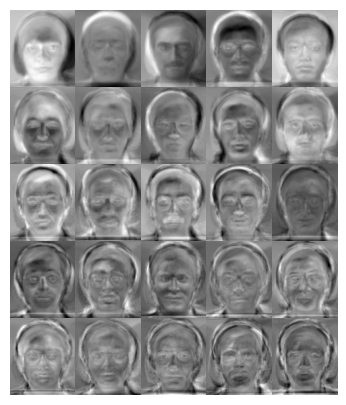
\includegraphics[width=0.8\textwidth]{figures/eigenfaces.png}
        \caption{The first 25 eigenfaces}
    \end{subfigure}
    % \hfill
    \begin{subfigure}{0.4\textwidth}
        \centering
        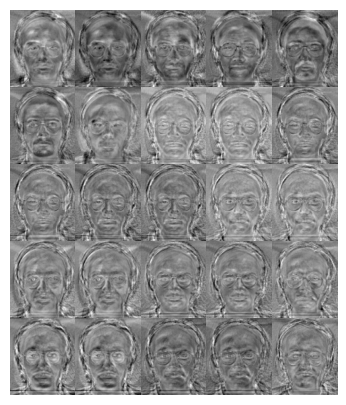
\includegraphics[width=0.8\textwidth]{figures/fisherfaces.png}
        \caption{The first 25 fisherfaces}
    \end{subfigure}
    \caption{Eigenfaces and Fisherfaces}
\end{figure}

Here is the randomly picked 10 images from the training/test set and their reconstructed images:

\begin{figure}[H]
    \centering
    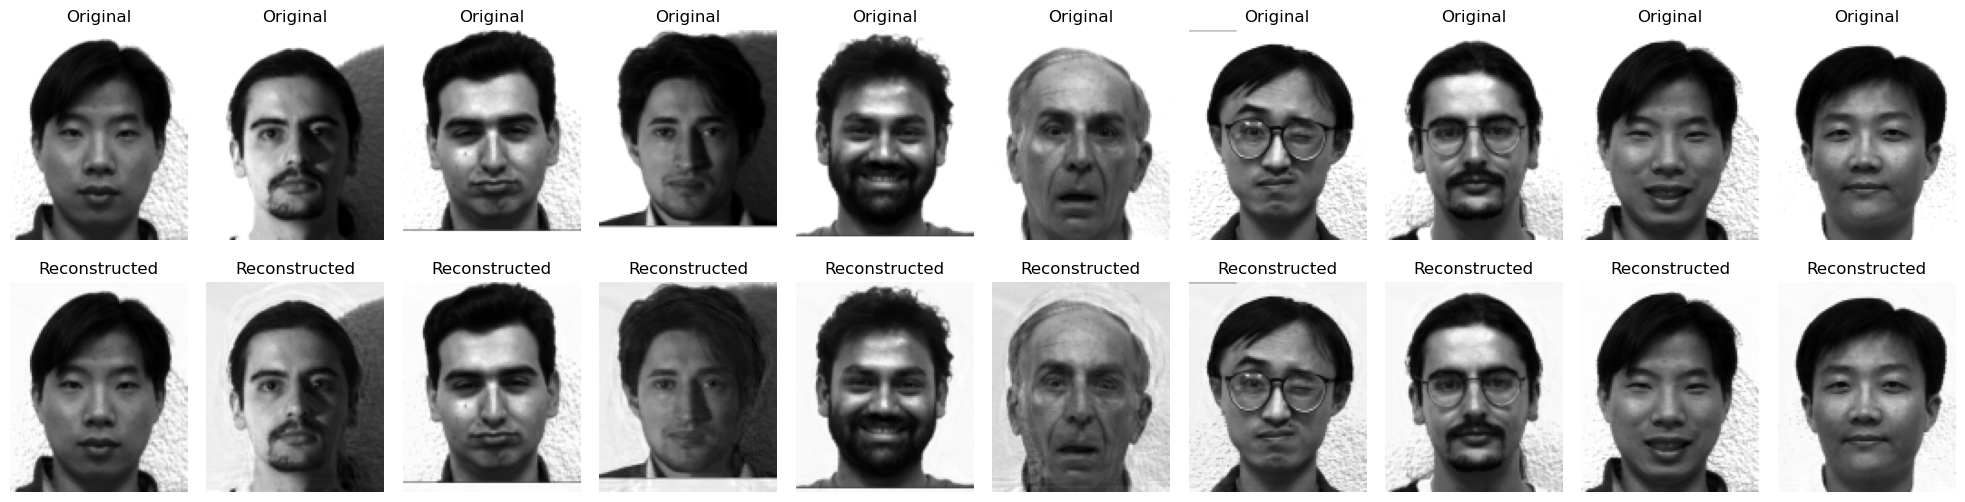
\includegraphics[width=0.8\textwidth]{figures/reconstructed_images_pca_training.png}
    \caption{Original and Reconstructed Training Images using PCA}
\end{figure}

\begin{figure}[H]
    \centering
    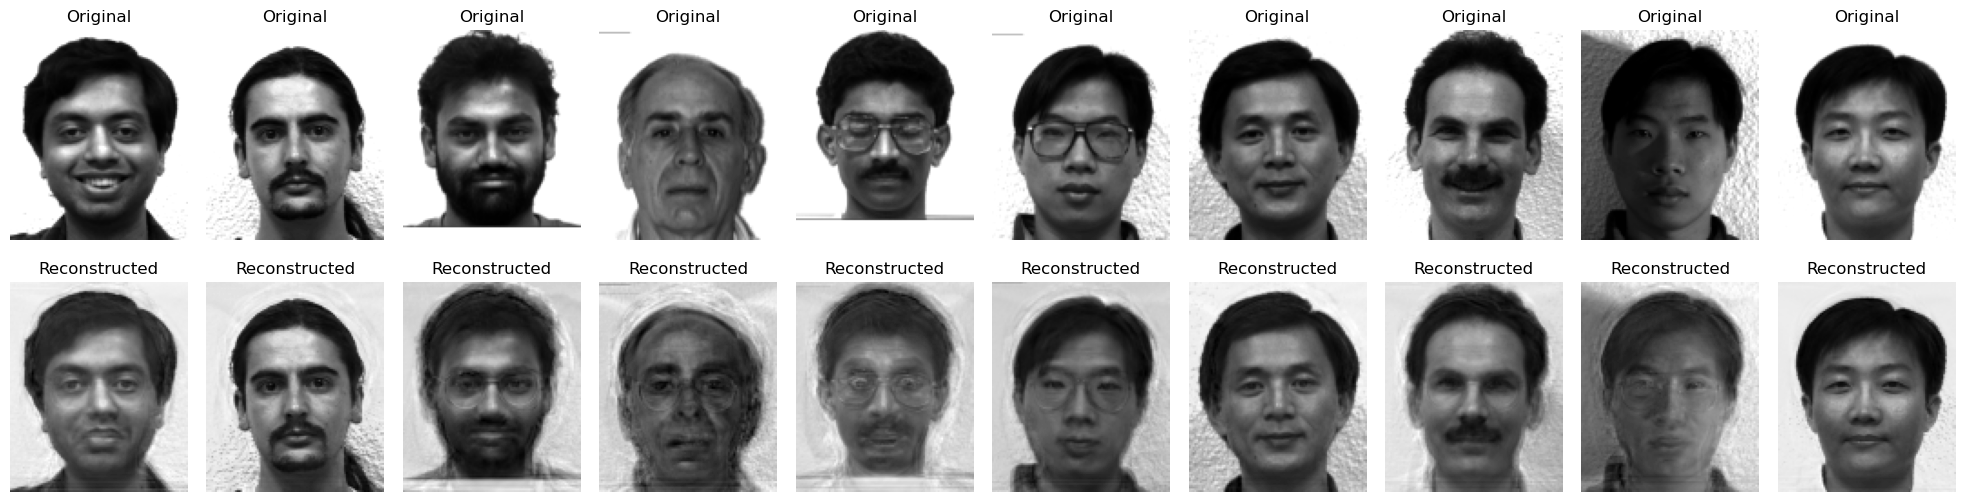
\includegraphics[width=0.8\textwidth]{figures/reconstructed_images_pca_testing.png}
    \caption{Original and Reconstructed Testing Images using PCA}
\end{figure}

\begin{figure}[H]
    \centering
    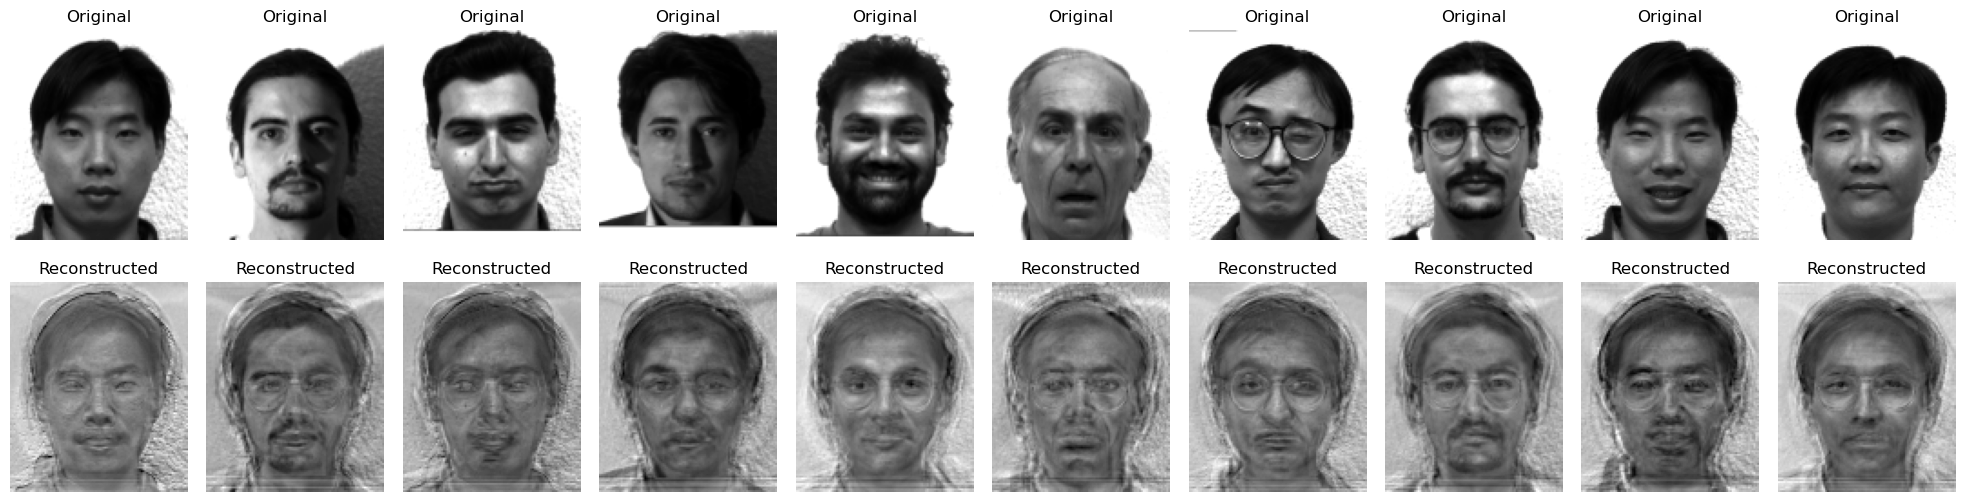
\includegraphics[width=0.8\textwidth]{figures/reconstructed_images_lda_training.png}
    \caption{Original and Reconstructed Training Images using LDA}
\end{figure}

\begin{figure}[H]
    \centering
    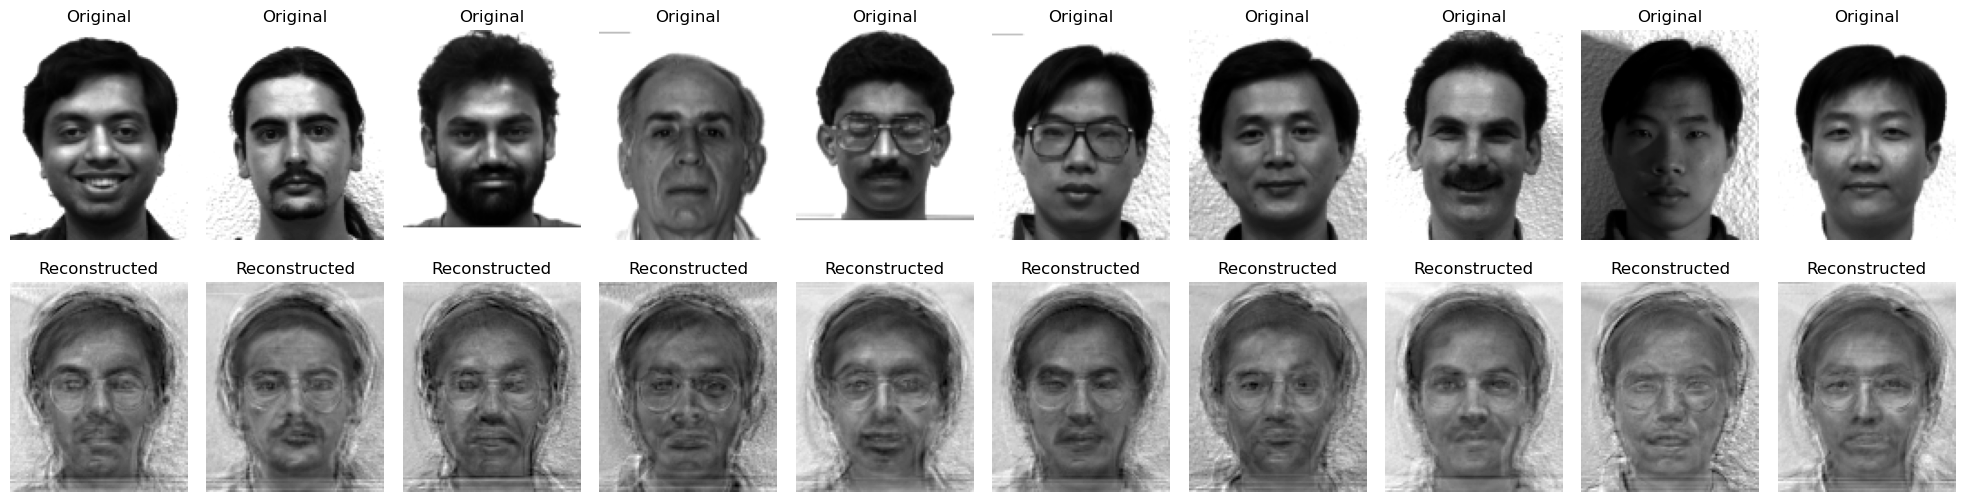
\includegraphics[width=0.8\textwidth]{figures/reconstructed_images_lda_testing.png}
    \caption{Original and Reconstructed Testing Images using LDA}
\end{figure}

\subsubsection{Part 2}

The accuracy of KNN on PCA and LDA is shown below:

\begin{table}[H]
    \centering
    \begin{tabular}{|c|c|}
        \hline
        Method & Accuracy \\
        \hline
        PCA & 0.83 \\
        LDA & 0.9 \\
        \hline
    \end{tabular}
    \caption{Accuracy of KNN on PCA and LDA}
\end{table}

\subsubsection{Part 3}

The accuracy of KNN on Kernel PCA and Kernel LDA is shown below:

\begin{table}[H]
    \centering
    \begin{tabular}{|c|c|c|}
        \hline
        Method & Kernel & Accuracy \\
        \hline
        PCA & QBF & 0.83 \\
        PCA & RBF ($\gamma=0.001$) & 0.83 \\
        LDA & QBF & 0.5 \\
        LDA & RBF ($\gamma=0.000001$) & 0.86 \\
        \hline
    \end{tabular}
    \caption{Accuracy of KNN on Kernel PCA and Kernel LDA}
\end{table}

We can see that the accuracy of LDA is the highest, but the accuracy of LDA with QBF kernel is the lowest, which might means that the QBF kernel is not suitable for LDA.

For PCA, the accuracy is the same for non-kernel, QBF ,and RBF kernel, which might means that the kernel function does not affect the performance of PCA.

But the accuracies are very similar because the testing dataset is small, leading to less stable accuracy measurements.

\subsection{t-SNE}

\subsubsection{Part 1}

The t-SNE and s-SNE results are shown below:

\begin{figure}[H]
    \centering
    \begin{subfigure}{0.4\textwidth}
        \centering
        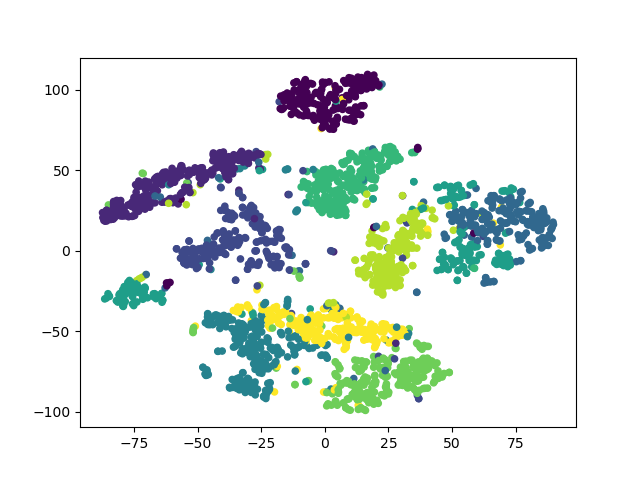
\includegraphics[width=0.8\textwidth]{figures/t-SNE.png}
        \caption{t-SNE}
    \end{subfigure}
    % \hfill
    \begin{subfigure}{0.4\textwidth}
        \centering
        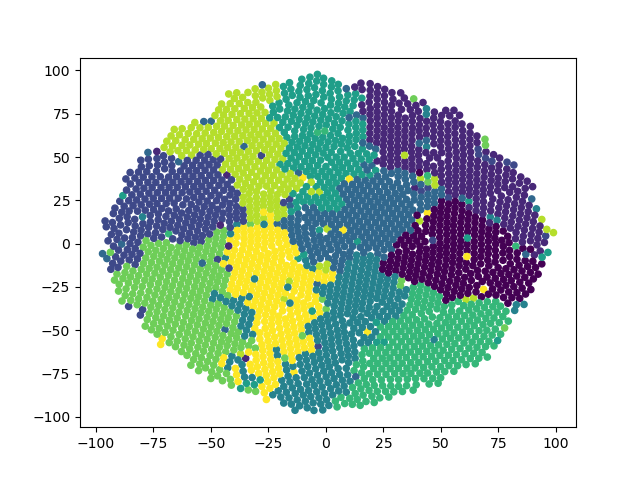
\includegraphics[width=0.8\textwidth]{figures/symmetric_SNE.png}
        \caption{s-SNE}
    \end{subfigure}
    \caption{t-SNE and s-SNE Results}
\end{figure}

We can see that the s-SNE result has the crowding problem, which is because the Gaussian kernel in the low-dimensional space allocates too much probability mass to nearby points, leaving insufficient space to represent moderately distant points.

As a result, global relationships in s-SNE are poorly preserved, and the data appears overly compacted.

\subsubsection{Part 2}

The animation of t-SNE and s-SNE optimization process is shown below (6 frames):

\begin{figure}[H]
    \centering
    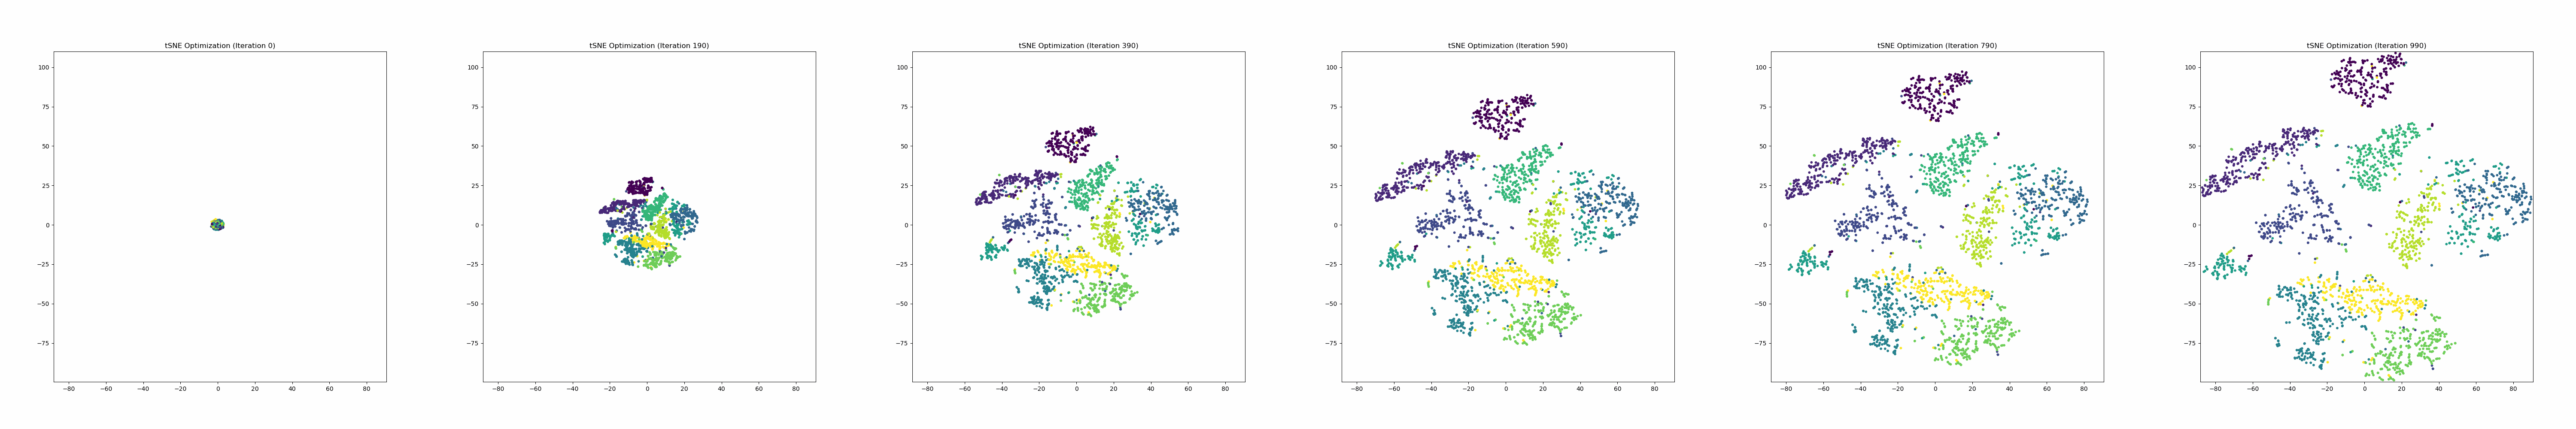
\includegraphics[width=1\textwidth]{figures/flatgif_tsne_animation.png}
    \caption{t-SNE Optimization Animation}
\end{figure}

\begin{figure}[H]
    \centering
    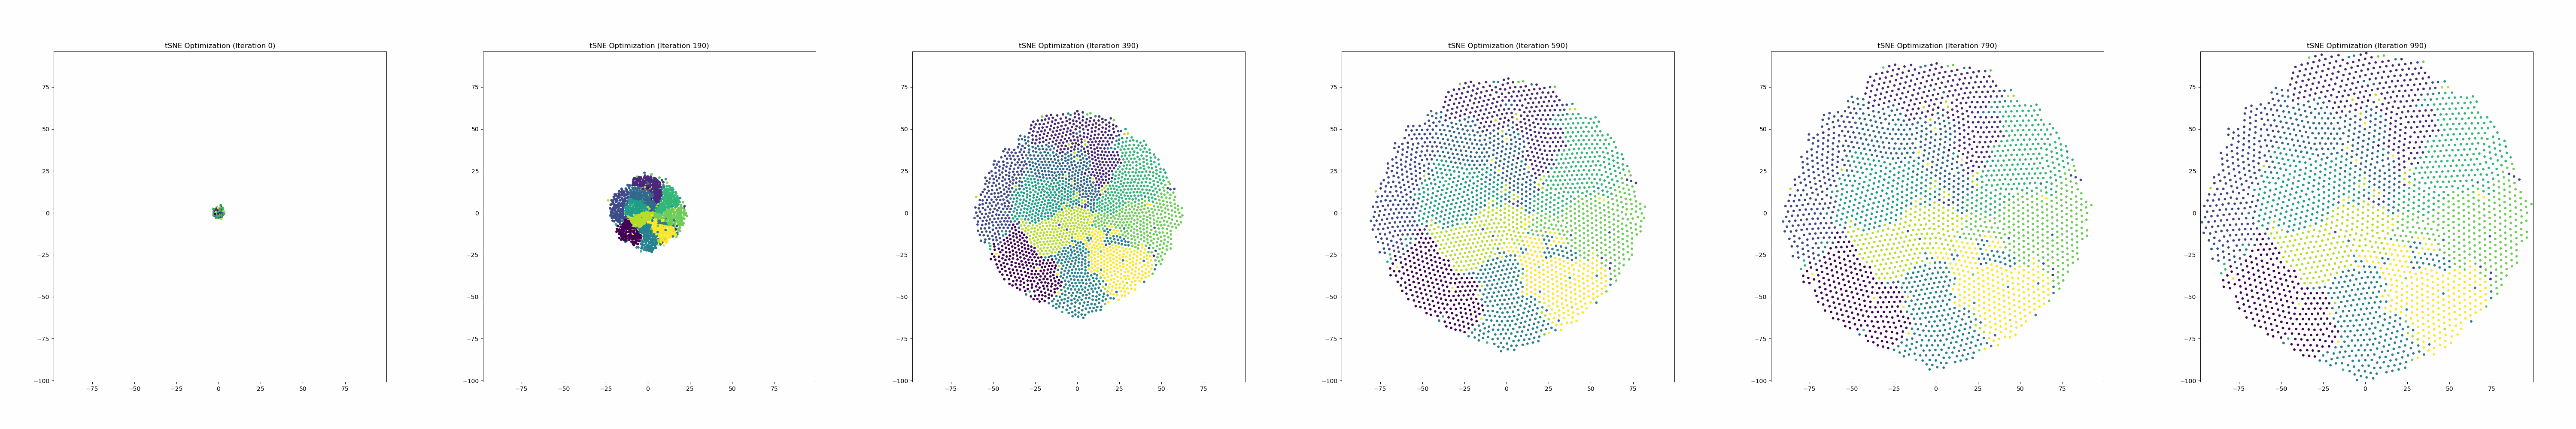
\includegraphics[width=1\textwidth]{figures/flatgif_symmetric_sne_animation.png}
    \caption{s-SNE Optimization Animation}
\end{figure}

We can see that the t-SNE process is more seperated than the s-SNE process, which is consistent with the results in the previous part.

\subsubsection{Part 3}

The distribution of pairwise similarities in high-dimensional space and low-dimensional space based on both t-SNE and symmetric SNE is shown below:

\begin{figure}[H]
    \centering
    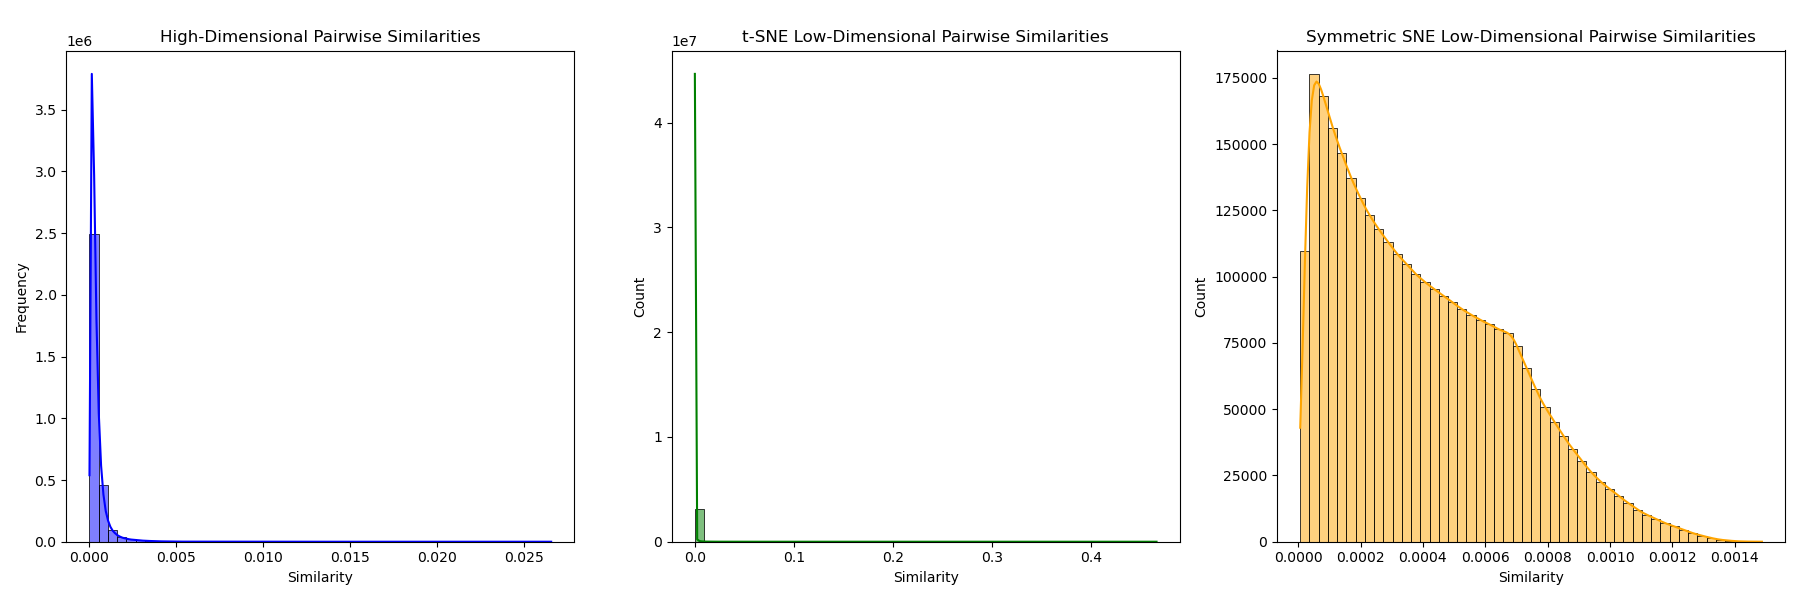
\includegraphics[width=1\textwidth]{figures/pairwise_similarities_distribution.png}
    \caption{Pairwise Similarities Distribution}
\end{figure}

\subsubsection{Part 4}

\section{Observations and Discussion}

The homework explored dimension reduction techniques like PCA, LDA, Kernel PCA, and Kernel LDA.

Eigenfaces and Fisherfaces provided meaningful insights into face recognition, significantly reducing computation time and enabling efficient KNN classification by lowering data dimensionality.

PCA achieved stable performance across kernels, while Kernel LDA demonstrated sensitivity to kernel choice, with RBF outperforming QBF.

The difference of t-SNE and s-SNE optimization highlighted its capacity to preserve local structures, whereas s-SNE suffered from crowding effects, impacting global data representation.

These findings emphasize the importance of selecting appropriate methods and parameters based on the dataset characteristics.

\end{document}